\subsection{Type \Rmnum{1} Events: Single Scattering Involving the Tip}
The most dominant features of weirdospace are known as {\it primary
stripes}.  Primary stripes are thought to arise from single scattering off
the tip.  Consider the phase accumulation for this event type.  It consists
of only two terms: the local phase $\varphi_\mathrm{l,tip}$ sampled by the tip
position $(x_\mathrm{tip},y_\mathrm{tip})$, and the phase to the far field
$\varphi_\mathrm{ff,tip}$.  The intensity in weirdospace for primary stripes is
\begin{align}
E_\mathrm{\Rmnum{1}}=
A_\mathrm{\Rmnum{1}}\;
e^{i(\varphi_\mathrm{l,tip}+\varphi_\mathrm{ff,tip})}
\end{align}
where an argument $a e^{i \Phi}$, representing is a fixed background phase required to
produce any structure at all is always assumed to be present.  As outlined in Bert's thesis, there is
excellent agreement between experiment and theory regarding the
mathematical description of this feature.

Observe Permutations \numrange{0}{7} in Figure \ref{fig:clevergridlinhsv}.  All of these include single
scattering off the tip and off of them exhibit primary stripes.  The
marginal exception is Permutation \num{5}, where primary stripes appear as
a phase rather than an intensity feature.  Nonetheless, primary stripes
appear in all permutations where single scattering off the tip is present, and
conversely are suppressed in all where it is not.

\subsection{Type \Rmnum{2} Events: Single Scattering not Involving the Tip}
Single scattering not involving the tip can be thought of as the
superposition of all single scattering events from all scatterers.
\begin{align}
E_\mathrm{\Rmnum{2}}=
\sum_{n=0}^{N}
A_{\mathrm{\Rmnum{2}},n}\;
e^{i(\varphi_{\mathrm{l},n}+\varphi_{\mathrm{ff},n})}
\end{align}
In the far field the superposition of many waves with phase terms
$\varphi_{\mathrm{l},n}$ and $\varphi_{\mathrm{ff},n}$, themselves
essentially uncorrelated and uniformly random tend to cancel each other out.
The result of this is a random fixed phase (white noise), shown singly in
Permutation \num{11}.

I don't quite have all the math down on this one yet.  If we assume the
total phase of the argument for this event type is modeled by a 
uniform random variable, then the real or imaginary part of the
exponential will also be a random variable $\in (-1,1)$.  This of course is
a random walk with an expectation value of $0$ (or very nearly such for a
finite number of waves).

\subsection{Type \Rmnum{3} Events: Multiple Scattering Involving the Tip}
This is where things get interesting.  Consider a multiply scattered path
involving the tip where the tip is {\bf not} the last scatterer.  The phase
to the far field $\varphi_\mathrm{ff}$ is determined by the superposition
of all the randomly placed scatterers, so it should behave like the phase
from a Type \Rmnum{2} event -- an essentially constant background.  The
local phase consists of many multiply scattered paths involving the tip,
the result of which is like adding a constant to the phase of the tip -- the
phase from all the paths not involving the tip average out and all you get
is the local tip phase.  This manifests itself in weirdospace as a fixed
background at the plasmon frequency (the ``horizontal bars'') as a wave of
the form
\begin{align}
E_\mathrm{\Rmnum{3}a}= A_\mathrm{\Rmnum{3}a}\;e^{i(k_\mathrm{sp}x)}
\end{align}
This can easily be seen in the \SI{180}{\degree} scattering direction for
all permutations which include multiple scattering involving the tip.
Also, note that only in cases where multiple scattering involving the tip
has been suppressed does this kind of background disappear.  

Again, here I haven't reached the result analytically, but numerical
estimates confirm that, say for an infinite sum of cosines and a random
variable $p_n$
\begin{align}
\lim_{N\to\infty}\sum_{n=0}^{N}\frac{\cos(r+p_n)}{N}=\cos(r+\vartheta)
\end{align}
where $\vartheta$ is a fixed phase.

Next, consider a multiply scattered path involving the tip where the tip is
the last scatterer.  The statistical result is similar to that of the
previous case, but here the local phase becomes a constant fixed phase and
the phase to the far field is all which is preserved.  This manifests
itself as a set of stripes of fixed wavelength, making a complete rotation
every rotation around the ring.  
\begin{align}
E_\mathrm{\Rmnum{3}b}=
A_\mathrm{\Rmnum{3}b}\;
e^{i k_\mathrm{sp}\left(x_n\cos\phi+y_n\sin\phi\right)}
\end{align}
At \num{0} and $\pi\;\si{\rad}$ these are indistinguishable from the previous
case, and orthogonal at $\pi/2$ and $3\pi/4 \;\si{\rad}$.  
It should be noted here that if the path involved the tip twice where the
tip occurs in both the local phase and the phase to the far field, this is
identical to a Type \Rmnum{1} event.

The combination of the two Type \Rmnum{3} events with the Type \Rmnum{1}
and \Rmnum{2} events explain much of the structure around the ring, as are
shown in the figures in the Appendix.

\subsection{Type \Rmnum{4} Events: Multiple Scattering Not Involving the Tip}
Somewhat anticlimactically, this results in another fixed background.  Both
the local phase and the phase to the far field are determined statistically
from the group as a whole in the same way as Type \Rmnum{2} events.

\subsection{Coherent Backscattering\\{\normalsize or}\\
Complex Exponentials and the Error of your Ways
\\{\normalsize or}\\
How I Learned to Stop Worrying and Love the Bomb
}
Since coherent backscattering (CBS) is a general multiple scattering
phenomenon, it was though that it would be seen in the experimental
weirdospace data - manifest as so called {\it secondary stripes}.  This
would be a wave identical to that of single scattering off the tip, but
excited by an evanescent field traveling in the opposite direction,
$\varphi_{\mathrm{l}}\to-\varphi_{\mathrm{l}}$.
\begin{align}
E_\mathrm{\chi}=A_\chi\;e^{i (-\varphi_{\mathrm{l}}+\varphi_{\mathrm{ff}})}
\label{eqn:cbs}
\end{align}
In Bert's thesis, the idea that secondary stripes were connected to CBS was
rejected based on analysis of the experimental data showing secondary
stripes were at the wrong angle.  I intend here to give evidence to the
contrary.

Figure \ref{fig:bertsdata1} shows the analytically predicted orientation of
secondary stripes along with the best fit orientation of such
stripes to an experimental weirdospace image for a particular angle along
the ring.  
\begin{figure}
\centering
\subfigure[expected]{
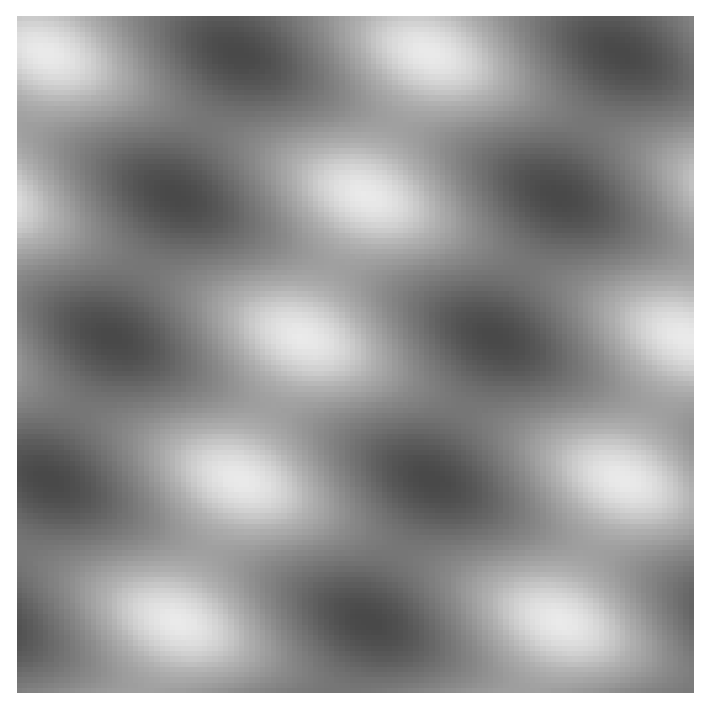
\includegraphics[width=3cm]{events/nuback-expected.eps}
}
\subfigure[best fit from experiment]{
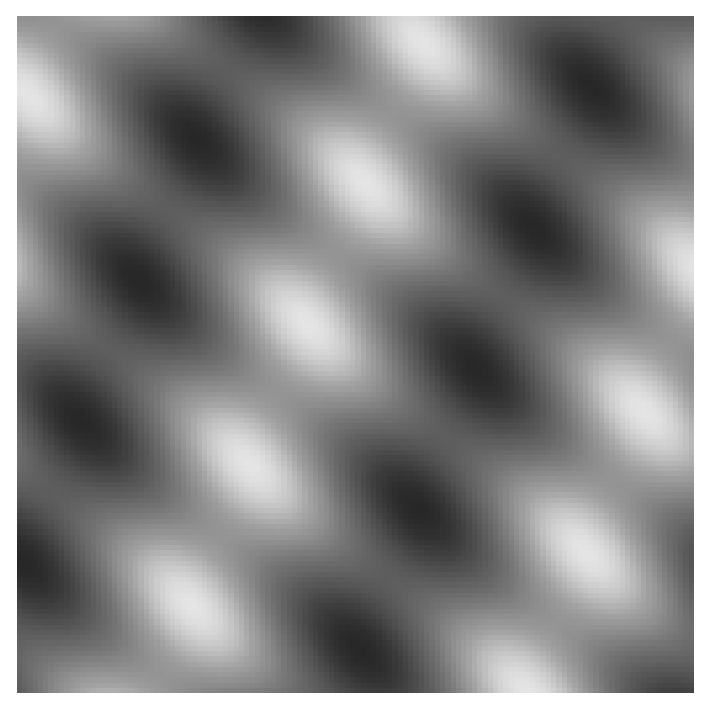
\includegraphics[width=3cm]{events/bestfit.eps}
}
\caption{Two figures from Bert's thesis.  To the left, the expected
orientation of secondary stripes and to the right, the best fit from the
experimentally measured orientation.}
\label{fig:bertsdata1}
\end{figure}
If you look carefully, you'll notice something strange about the figure:
the secondary stripes almost perfectly ``line up''.  This is consistent
with one computing the intensity as the sum of the squares rather then the
square of the sums, the later befitting for wave superposition.  This is
detailed in Figure \ref{fig:sumsq}.  Here we show the approximate
orientation of primary and secondary stripes for the experimental data in
question along with the resultant sum of squares and square of sums.  In
this image, the difference between the two is marginal.  Indeed, a priori
interpretation of the images would not lead one to think they were anything
but inconsistent with the experiment.  However, by adjusting the relative
amplitudes of these waves as in Figure \ref{fig:increaseintensity},
assuming $E_\chi$ to be much less than $E_\mathrm{\Rmnum{1}}$, the analytic result
comes to match the experiment nearly perfectly.  It should be noted that
the figure in Bert's thesis shows a CBS signal about $1/3$ the amplitude of
single scattering off the tip, which doesn't seem to fit well with what one
would assume for such an effect.

There are many more examples of secondary stripes and their relation to
experiment in the Appendix.

\begin{figure}
\centering
\subfigure[$e^{i \alpha}$]{ % primary stripes

\includegraphics[width=3cm]{events/primaryonly.eps}
}
\subfigure[$e^{i \beta}$]{ % secondary stripes
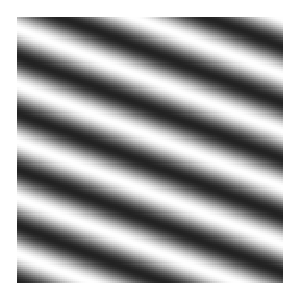
\includegraphics[width=3cm]{events/secondaryonly.eps}
}
% sum of squares
\subfigure[$\left|e^{i \alpha}\right|^2 + \left|e^{i \beta}\right|^2$]{
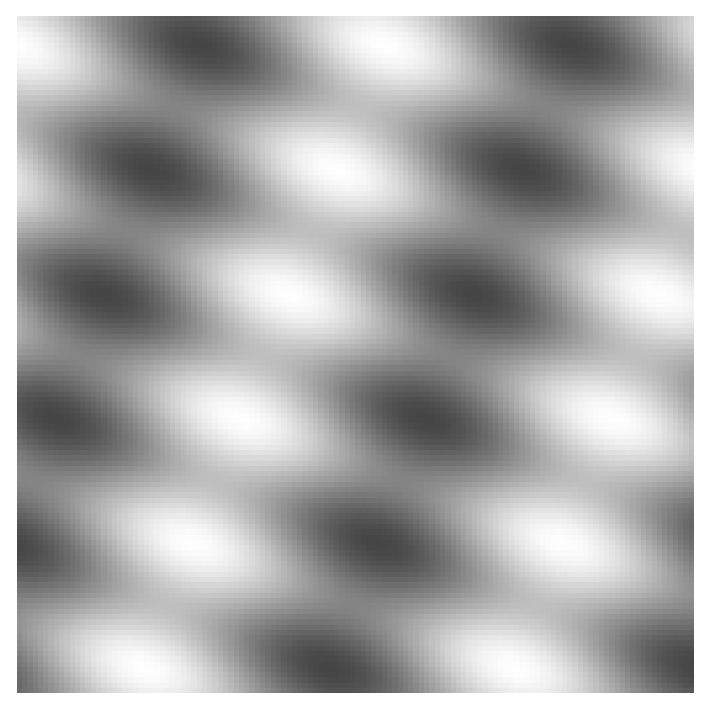
\includegraphics[width=3cm]{events/sumsq.eps}
}
% square of sum
\subfigure[$\left|e^{i \alpha} + e^{i \beta}\right|^2$]{
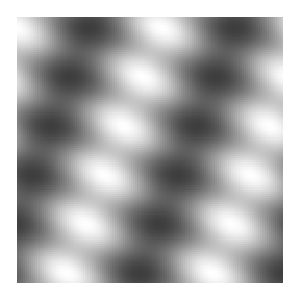
\includegraphics[width=3cm]{events/primaryplussecondary1.eps}
}
\caption{Adding phases from primary and secondary stripes results in a
characteristic interference pattern not consistent with the addition of
intensities.}
\label{fig:sumsq}
\end{figure}

\begin{figure}
\centering
\subfigure[$\left|0.29\cdot E_\mathrm{\Rmnum{1}} + 0.08\cdot E_\chi \right|^2$]{
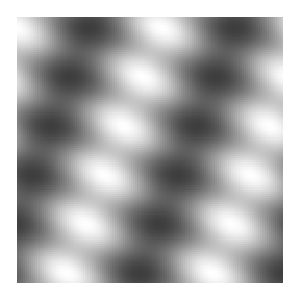
\includegraphics[width=3cm]{events/primaryplussecondary1.eps}
}
\subfigure[$\left|2.44\cdot E_\mathrm{\Rmnum{1}} + 0.23\cdot E_\chi \right|^2$]{
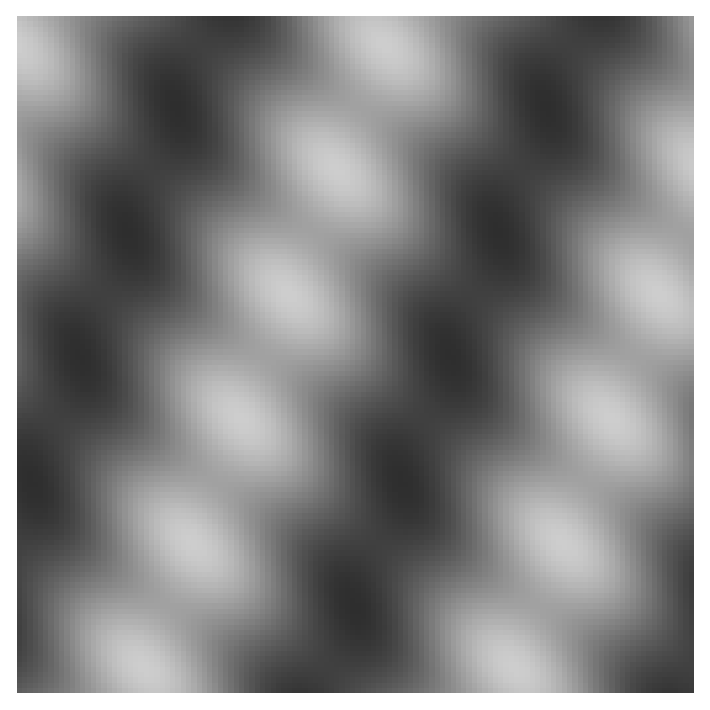
\includegraphics[width=3cm]{events/primaryplussecondary2.eps}
}
\subfigure[experiment]{
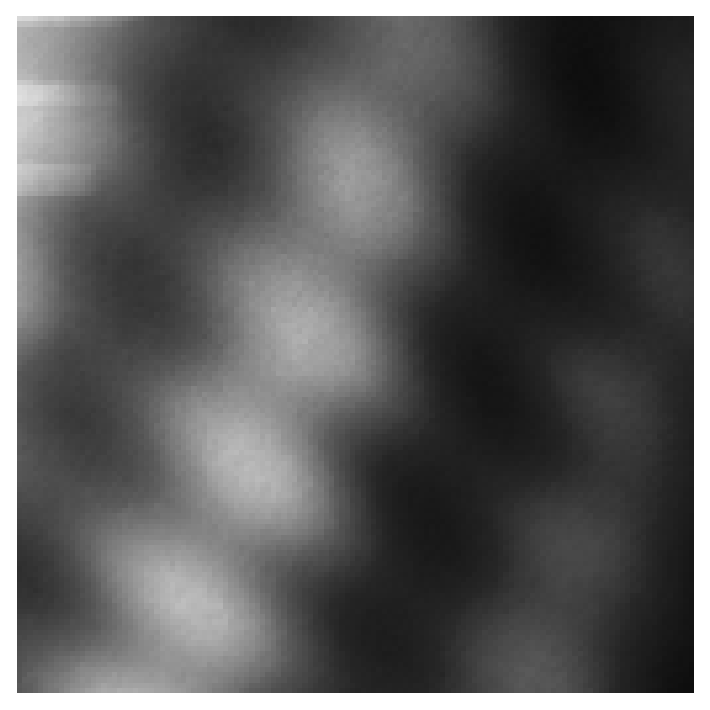
\includegraphics[width=3cm]{events/cbsstripedata.eps}
}
\caption{By adjusting the relative amplitudes of the waves predicted for
primary and secondary stripes, good agreement can be reached with the
experimental data.}
\label{fig:increaseintensity}
\end{figure}
We've actually seen this before in the Monte Carlo simulations, but didn't
know what to make of it without an explanation of the weirdospace features
caused my multiple scattering.  Figure \ref{fig:rtr} shows the difference
between analytic, with $E_\chi$ removed, and Monte Carlo simulations with
time reverse paths removed.  The results are almost exactly what one would
expect if secondary stripes were truly a coherent backscattering
phenomenon.  Amazing.
